\chapter{Mathematical Model}

\addcontentsline{toc}{chapter}{Mathematical Model}

\section{Model Description}

We are going to observe a mathematical model proposed by \cite{lips}, which describes the epidemiology of antimicrobial resistant infections in hospitals. The model examines a population of people in a closed environment, where new patients come into the system at some rate and go out of the system respectively. The model can be applied for the diseases that are transmitted through the skin, respiratory or digestive organs. A few examples of such bacteria are Escherichia coli, Staphylococcus, Enterococcus, Klebsiella pneumoniae and others. The mentioned bacteria are dangerous enough to cause a painful or even lethal infection. The hospital environment was chosen because the transmission of these bacteria often takes place inside the hospitals. Different patients may accidentally contact with each other and spread their infections to one another, as well as to medical personnel. The medical workers are also often responsible for the spread of infections inside the hospital, since they may pass the bacteria between their patients. This might happen as a result of insufficient hygiene with respect to their hands and inventory items. The bacteria in the system are continuously encountering the antibiotics that are used in the hospital. As a result, the patients may always get infected accidentally and the bacteria can pass their antibiotic resistant plasmids to other strains.

The model observes the transmission dynamics of the bacteria in a hospital, with regard to the usage of two different antibiotics - drug A and drug B. Some portion of all individuals that enter the hospital are already colonized with the bacteria, that we are looking at. The differential equations for the model will look as follows:

\begin{equation}
\frac{dS}{dt} = m \mu + \beta S X - (\tau_1 + \tau_2 + \gamma + \mu) S
\end{equation}

\begin{equation}
\frac{dR}{dt} = \beta (1 - c) R X - (\mu + \tau_2 + \gamma) R
\end{equation}

\begin{equation}
\frac{dX}{dt} = (1 - m) \mu + (\tau_1 + \tau_2 + \gamma) S + (\tau_2 + \gamma) R - \beta S X - \beta (1-c) R X - \mu X.
\end{equation}

$S$ in the equations, denotes the individuals that are infected with the bacteria sensitive to drug A. $R$ is correspondingly stands for the population infected with the bacteria resistant to drug A. By $X$ we denote the people who are not carrying any type of these bacteria. Also, it is assumed that there are no any bacteria resistant to drug B in the system. A fraction $m$ of people entering the bacteria is infected by a sensitive strain; the other $1-m$ of incoming people are not colonized with the bacteria at all ($X$).

\section{Model Implementation Platform}

AnyLogic is a multi-method simulation modeling tool developed by XJ Technologies.
The tool was named AnyLogic, because it supported all three well-known modeling approaches: System dynamics, Discrete event simulation, Agent-based modeling.

AnyLogic models can be based on any of the main simulation modeling paradigms:discrete event or process-centric (DE),systems dynamics (SD), and agent-based(AB)

\begin{figure}
   \centering
	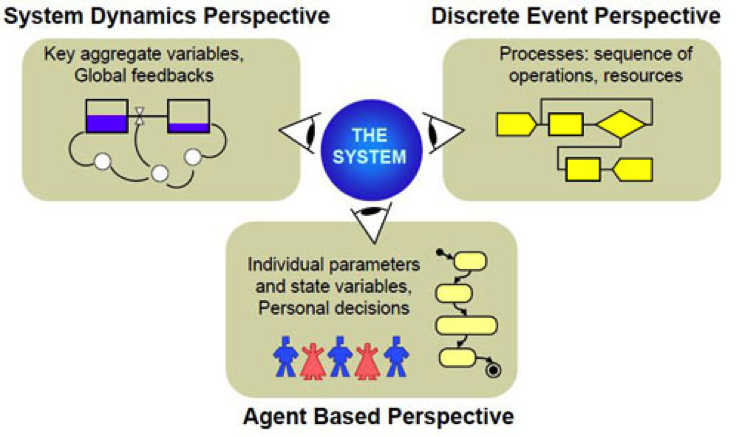
\includegraphics[width=0.9\textwidth]{img/system}
	\caption[Clear]{Modeling aproaches}
\end{figure}

System dynamics and discrete event are traditional simulation approaches, agent based is new. Technically, the system dynamics approach deals mostly with continuous processes whereas "discrete event" (by which we mean all descendants of GPSS also known as process-centric simulation approach) and agent based models work mostly in discrete time, i.e. jump from one event to another.

System dynamics and discrete event simulation historically have been taught at universities to very different groups of students, namely management and economy, industrial and operation research engineers. As a result, there are two distinct practitioners' communities that never talk to each other.

Agent based modeling until recently has been mostly a purely academic topic. However, the increasing demand for global business optimization caused leading modelers looking at combined approaches to gain a deeper insight into complex interdependent processes having very different natures.

AnyLogic includes a graphical modeling language and also allows the user to extend simulation models with Java code. The Java nature of AnyLogic lends itself to custom model extensions via Java coding as well as the creation of Java applets which can be opened with any standard browser. These applets make AnyLogic models very easy to share or place on websites. In addition to Java applets the Professional version allows for the creation of Java runtime applications which can be distributed to users. These pure Java applications can be a base for decision support tools System dynamics dealing with aggregates is obviously used at the highest abstraction level. Discrete event modeling is used at low to middle abstraction. As for agent based modeling, this technology is used across all abstraction levels, and agent may model objects of very diverse nature and scale: at the "physical" level agents may be e.g. pedestrians or cars or robots, at the middle level – customers, at the highest level – competing companies.

AnyLogic allows the modeler to combine these simulation approaches within the same model. There is no fixed hierarchy (see Figure 5). So, as an example, one could create a model of the package shipping industry where carriers are modeled as agents acting/reacting independently whereas the inner workings of their transport and infrastructure networks could be modeled with discrete event simulation. Similarly, one can model consumers as agents whose aggregate behavior feed a systems dynamics model capturing flows such as revenues or costs which do not need to be tied to individual agents. This mixed language approach is directly applicable to a wide variety of complex modeling problems that may be modeled via any one approach albeit with compromises.
